\documentclass[a4paper,17pt]{extarticle}
\usepackage[pdftex]{color,graphicx,epsfig}
\usepackage[final]{pdfpages}
\usepackage[francais]{babel}
\usepackage{graphicx}
\usepackage[T1]{fontenc}
\usepackage{textcomp}
\usepackage[utf8]{inputenc}
\usepackage{bookman}
\usepackage[T1]{fontenc}
\usepackage{fancybox}
\usepackage{tikz}
\usetikzlibrary{calc}

\graphicspath{ {../img/} }

\pagenumbering{gobble}

\def\blankpage{%
      \clearpage%
      \thispagestyle{empty}%
      \addtocounter{page}{-1}%
      \null%
      \clearpage}

\begin{document}

\title{Mirèlha}
\author{Frédéric Mistral}

% ---------------------
\begin{titlepage}

    \begin{tikzpicture}[remember picture, overlay]
      \draw[line width = 4pt] ($(current page.north west) + (1in,-1in)$) rectangle ($(current page.south east) + (-1in,1in)$);
    \end{tikzpicture}

        \begin{center}

        % Upper part of the page
        \textsc{\Huge Mirèlha}\\[1.5cm]

        \textsc{\Large Frederic Mistrau}\\[2.5cm]

        \includegraphics[width=0.65\columnwidth]{saintes_maries}
        \end{center}

        \vfill

\end{titlepage}

\newpage

\blankpage

\blankpage

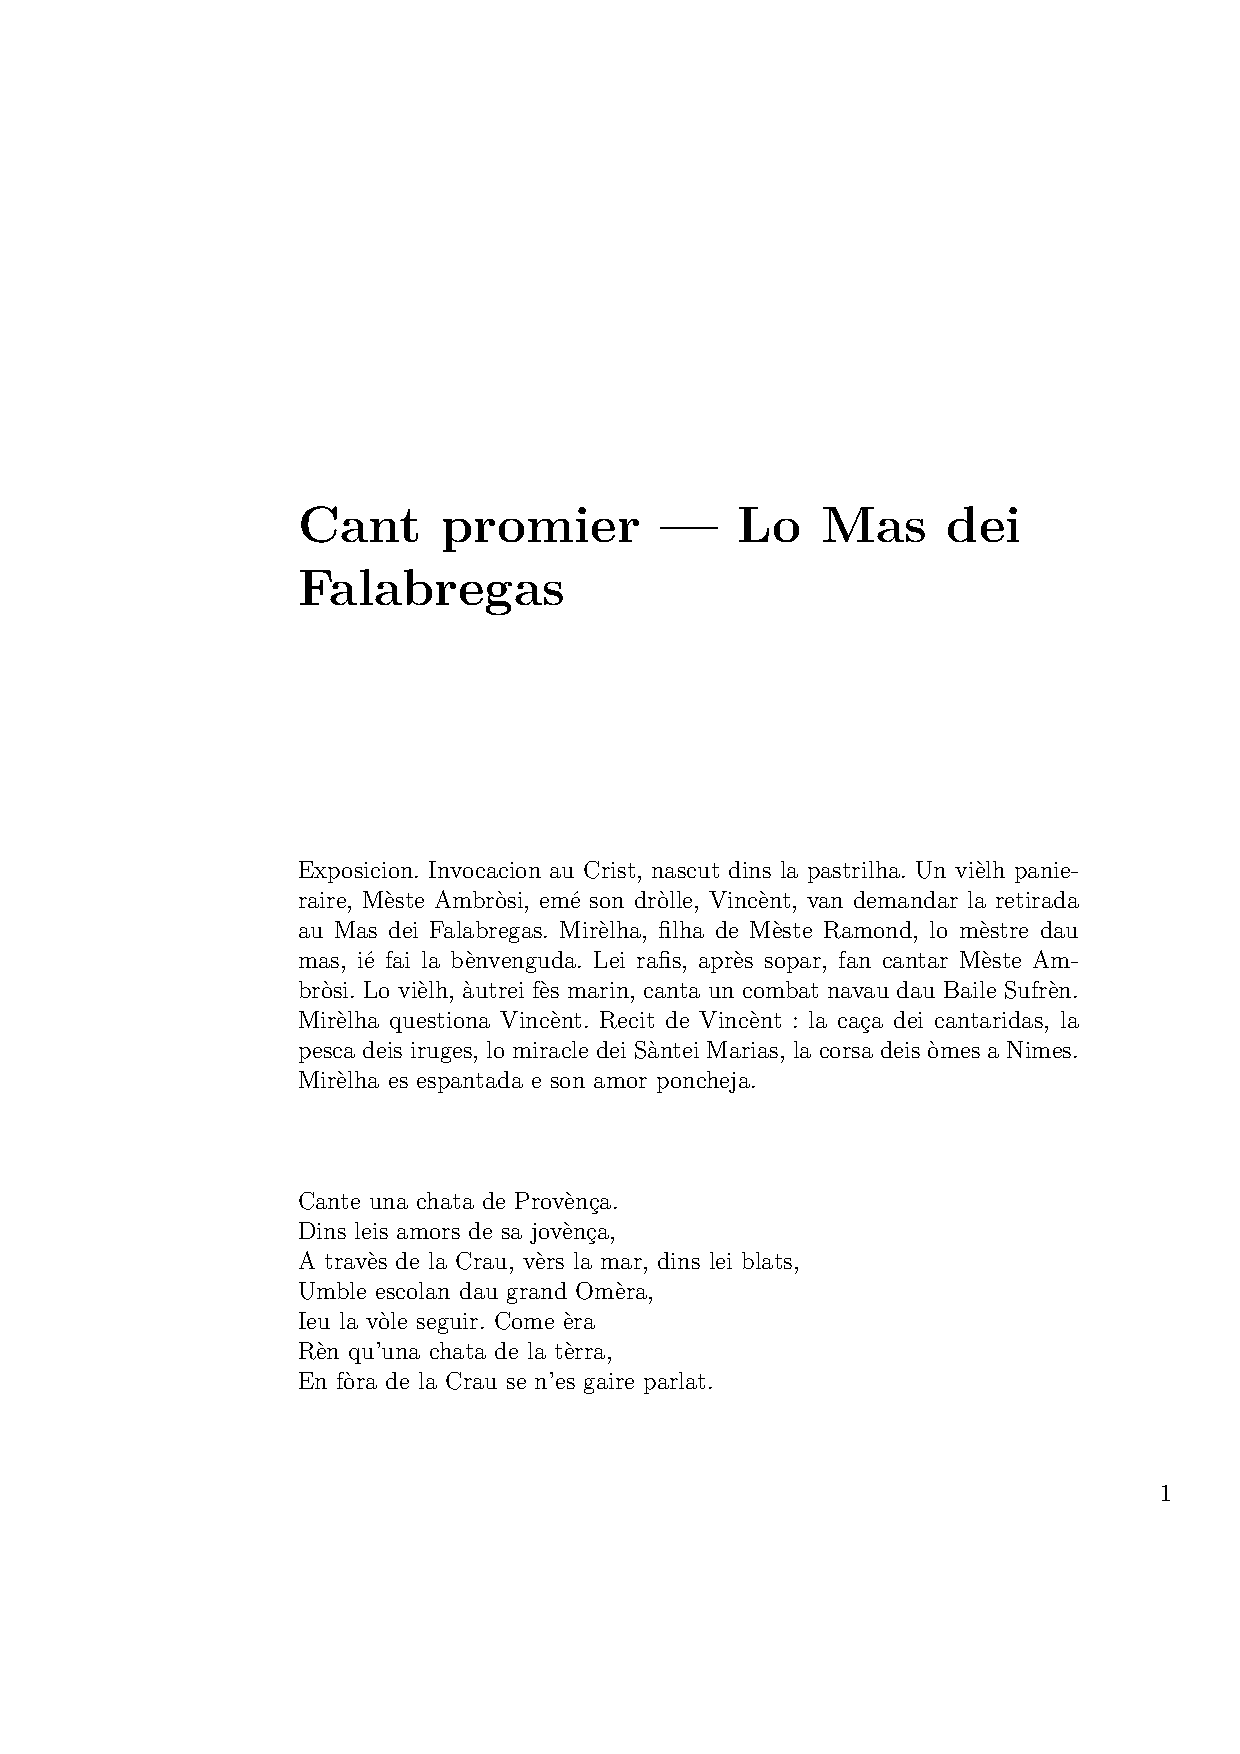
\includepdf[pages=-]{./halfparallelfiles.pdf}

\blankpage

\blankpage

\blankpage

\blankpage

\newpage

\begin{tikzpicture}[remember picture, overlay]
      \draw[line width = 4pt] ($(current page.north west) + (1in,-1in)$) rectangle ($(current page.south east) + (-1in,1in)$);
\end{tikzpicture}

\begin{center}
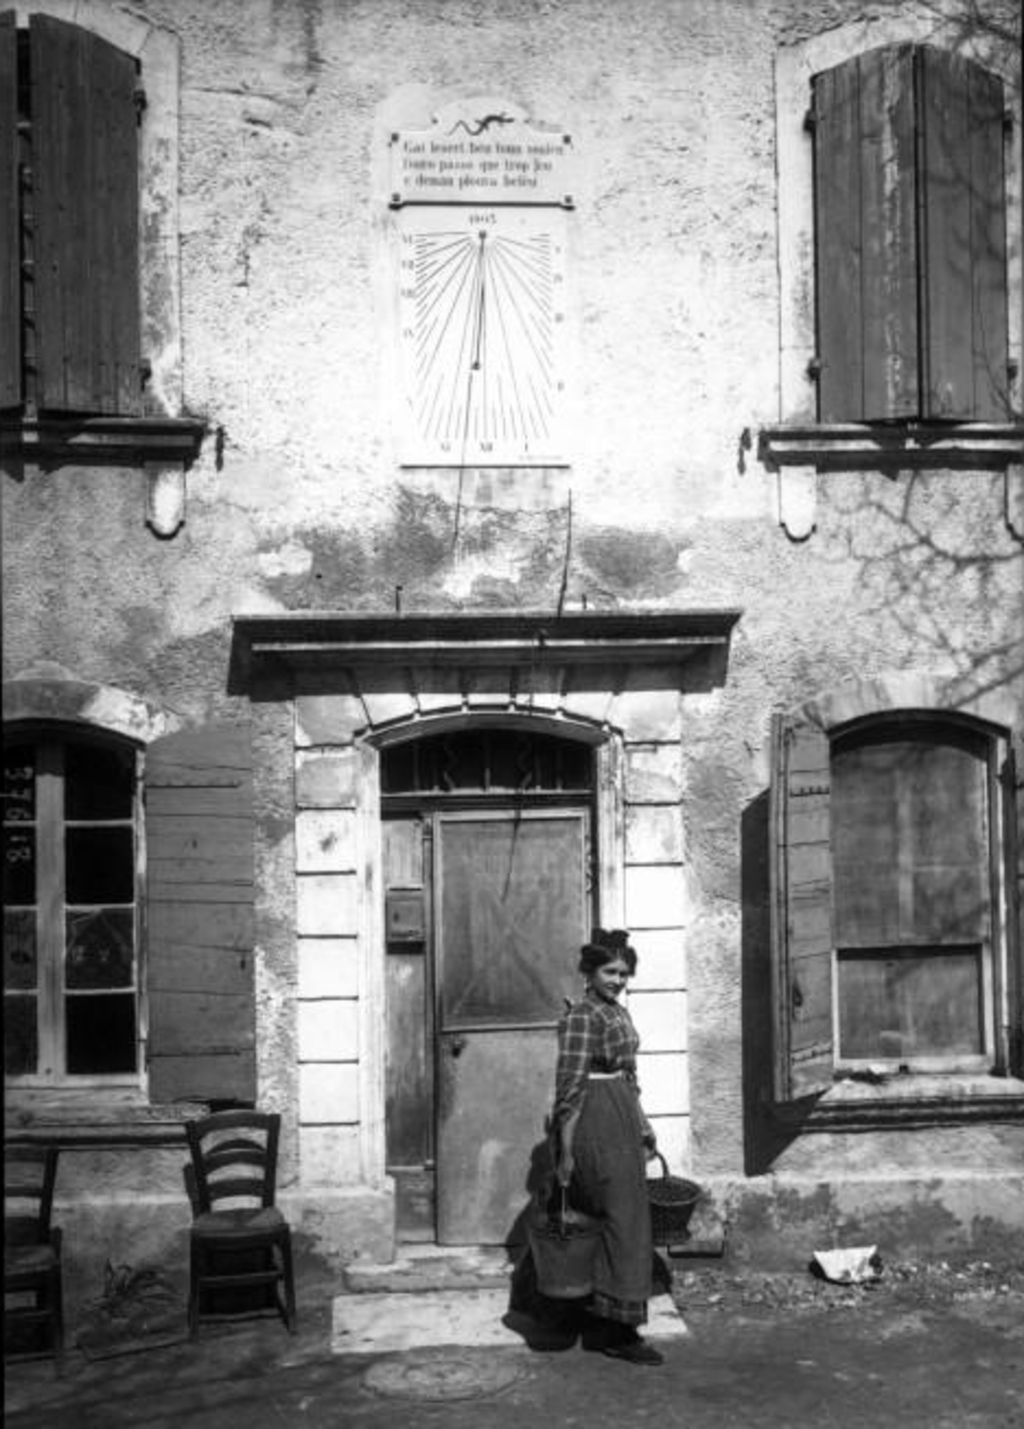
\includegraphics[width=0.65\columnwidth]{ostau.jpg}\\[2.0cm]

{\small Cante una chata de Provènça...}\\[2.0cm]

\end{center}

\end{document} 
